%!TEX root = ../msc_thesis.tex

\chapter{Theoretical Framework}
\label{ch:theory}


\section{Related work}

As mentioned before, Bayesian Artificial Neural Networks date back to late 1980s and early 1990s. These first approaches focused on Markov Chain Monte Carlo (MCMC) as the main method get samples of the posterior distribution of the parameters. Lately, there's been more work in the area, such as the Probabilistic Backpropagation algorithm developed by \citeauthor{hernandez2015probabilistic}, which relies on one-dimensional Gaussian distributions that approximate the marginal posterior distribution of the weights on each iteration of backpropagation \cite{hernandez2015probabilistic}. There is also the work by \citeauthor{graves2011practical}, based on variational inference to approximate the posterior distribution of the parameters \cite{graves2011practical}. These methods, however, do not scale well to very big network architectures and datasets; and they also have the disadvantage that they only work with multi-layer perceptron architectures, making them impossible to use with more recent architectures such as Convolutional Neural Networks (CNNs) or Recurrent Neural Networks (RNNs).

Recently, \citeauthor{gal2015dropout1} showed that a neural network with arbitrary depth, with dropout applied before each weight layer, is equivalent to the variational approximation to a deep Gaussian process. This is because the loss function minimizes the Kullback-Leibler divergence between an approximate distribution and the posterior of a deep Gaussian process \cite{gal2015dropout1}. This means that we can get uncertainty estimates with the models already trained with dropout without changing anything during training, the only difference comes at prediction time in which instead of doing a single forward pass and multiply each layer by a weight proportional to dropout probability, we just do several forward passes with dropout. They also showed in \cite{gal2015modern} that stochastic regularization techniques in arbitrary neural models can be seen as approximate variational inference in Bayesian Neural Networks.

This work is further extended by the same authors and they showed that the same ideas of dropout as a Bayesian approximation can be used in CNNs \cite{gal2015bayesian}. In particular, the showed that dropout can be seen as approximate variational inference in Bayesian Neural Networks, thus permitting the use of operations such as convolution and pooling in probabilistic models. The implementation is reduced to performing dropout after each convolution layer at training, and by performing several stochastic forward passes through the model (same idea as before). These stochastic forward passes are referred to as Monte Carlo (MC) dropout. Dropout is not usually performed after convolutional layers because it does not seem to give any benefits, but \citeauthor{gal2015bayesian} show empirically that MC-dropout can help with overfitting.

The work on CNNs is then used in an Active Learning environment, where the goal is to label images intelligently so that a model has good performance with a lower number of training examples \cite{Gal2016Active}. Deep learning poses several difficulties when used in an Active Learning setting because, first, small amounts of data need to be handled; and second, many Active Learning acquisition functions rely on model uncertainty, which is rarely represented in Deep Learning. \citeauthor{Gal2016Active} are able to achieve 5\% test error on the MNIST dataset with only 295 labeled images without, and 1.64\% test error with 1000 labeled images. They compare five different acquisition functions: choosing images that maximize the predictive entropy (Max Entropy); the ones that maximize the mutual information between predictions and model posterior (BALD); the ones that maximize the Variation Ratios; the ones that maximize mean standard deviation; and random acquisition (baseline). They also compare it with deterministic CNNs which, like the Bayesian CNN, produce a probability vector which can be used with the acquisition functions, but the Bayesian models, propagating uncertainty throughout the model, attain higher accuracy early on, and converge to a higher accuracy overall.

The dropout variational approach can also be used in Recurrent Neural Networks (RNNs), as shown by \citeauthor{gal2016theoretically} in \cite{gal2016theoretically}. In this paper, the authors give insight on how to use dropout with RNNs (something seldom done) and apply it on LSTM and GRU models, outperforming existing techniques in language modeling with the Penn Treebank dataset.

An example of how the uncertainties provided by Bayesian Neural Networks can be used, is shown by \citeauthor{li2017dropout} in \cite{li2017dropout}. They use adversarial examples and check if they can be told apart by examining the uncertainty representation of the dropout models. The deterministic Neural Networks produce over-confident predictions on these adversarial samples (they predict the wrong label very confidently), while dropout models, though producing wrong labels, are very uncertain about their predictions. They finish by stating that their results suggest that assessing the uncertainty of classification models can be used to identify adversarial examples, but much more research is needed to solve the difficulties faced with adversarial inputs.

The research on adversarial examples is continued by \citeauthor{rawat2017adversarial}, who study different Bayesian approaches (Bayes by Backprob (BBB), Probabilistic Backpropagation (PBP), Variational Matrix Gaussian (VMG) and MC-Dropout) and the uncertainty provided by the models, and prove that these models exhibit increased uncertainty when under attack \cite{rawat2017adversarial}. They state that all of the architectures in their study are Multi-Layer Perceptron, which do not scale for high dimensional colored images, with the exception of MC-Dropout, and therefore, a detailed study for MC-Dropout is required to demonstrate the applicability of model uncertainty for adversarial detection on various state-of-the-art attacks.

\section{Artificial Neural Networks}

The most basic, and perhaps the best known, type of Artificial Neural Network (ANN) is called a feedforward neural network or multilayer perceptron (MLP). These models are basically a composition of non-linear functions of the data. Let's illustrate this with a simple example.

Consider that we want to model a continuous variable $y$ from a single covariate $x$. A very simple model would be a linear regression, which models each observation $i$ as $y_i = \beta_0 + \beta_1 x_i$, and chooses the values of $\beta_0$ and $\beta_1$ that minimize some error function. ANNs go further and take non-linear transformations of this linear predictor with some function $\sigma(\cdot)$, such that $y_i = \theta_0 +  \sum_{k = 1}^m \theta_k \sigma \left( \beta_0^{k} + \beta_1^{k} x_i \right)$, where $m$ is manually chosen beforehand. A common choice for $\sigma(\cdot)$, which is called the \textbf{activation function}, is the logistic function $\sigma(x) = (1 + e^{-x})^{-1}$
or the hyperbolic tangent $\tanh(\cdot)$. The values of parameters $\theta_k$ and $\beta_j^{k}$ for $k \in \left\{ 0, \ldots, m \right\}$ and $j \in \left\{ 0, 1 \right\}$ are also chosen to minimize certain error function. Figure \ref{fig:theory_ANN_diagram_01} shows these relationships in a graphic way for a model with $m = 3$ and where we define $a_{k} = \sigma \left( \beta_0^{k} + \beta_1^{k} x_i \right)$ for $k \in \left\{ 1, 2, 3 \right\}$.
This image doesn't explicitly show the parameters $\beta_0^{k}$ for $k \in \left\{ 0, \ldots, m \right\}$, which are usually called the \textbf{bias} parameters.

\begin{figure}[H]
    \centering
    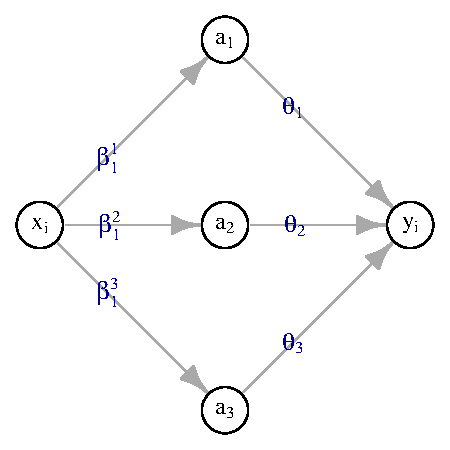
\includegraphics[width=0.5\textwidth]{plot_ANN_01.pdf}
    \caption{Diagram of a multilayer perceptron with $m = 3$.}
    \label{fig:theory_ANN_diagram_01}
\end{figure}

If the response variable $y$ happened to be a categorical variable, let's say binary, then one last transformation would have to be applied to map the model to the $\left[0, 1\right]$ interval and model $y$ as a probability. Then we would have

$$
y_i =
\phi \left( \theta_0 +  \sum_{k = 1}^p \theta_k \sigma \left( \beta_0^{k} + \beta_1^{k} x_i \right) \right) =
\phi \left( \theta_0 +  \sum_{k = 1}^p \theta_k a_{k} \right),
$$

with $\phi(\cdot)$ the logistic function to map from $\mathbb{R}$ to $\left[ 0, 1 \right]$. The choice of function $\phi(\cdot)$ depends on the nature of the response variable. As we saw previously, in the case of a continuous response variable, $\phi(\cdot)$ is the identity function.

We can establish a more complex model by taking linear combinations of non-linear functions of the previous result. In this case, we must add one more index to the $\theta$ parameters to keep using the same notation. Let's define
$$
a_k^{[1]} = \sigma^{[1]} \left( \beta_0^{k} + \beta_1^{k} x_i \right)
$$

for $k \in \left\{ 1, \ldots, m \right\}$ and

$$
a_k^{[2]} = \theta_0^{j} +  \sum_{k = 1}^m \theta_k^{j} \sigma^{[2)} \left( \beta_0^{k} + \beta_1^{k} x_i \right) =
\theta_0^{j} +  \sum_{k = 1}^m \theta_k^{j} a_k^{[1]}
$$

for $j \in \left\{ 1, \ldots, r \right\}$, then

$$
y_i = w_0 + \sum_{l = 1}^r w_j \sigma^{[2]} \left( a_j^{[2]} \right),
$$

where $r$, like $m$, is chosen beforehand. The values $m$ and $r$ are usually called the number of nodes or units of each layer. This is what is called a deeper model, because it has more layers. Notice that we have two different activation functions $\sigma^{[1]}(\cdot)$ and $\sigma^{[2]}(\cdot)$. Each layer can have a different function. The first one could be a sigmoid function and the second one a hyperbolic tangent, or vice versa, or they could both be the same function.

Figure \ref{fig:theory_ANN_diagram_02} shows this graphically with $m = 3$ and $r = 2$. Layers corresponding to $a_k^{[1]}$ and $a_j^{[2]}$ are called the \textbf{hidden layers}. So figure \ref{fig:theory_ANN_diagram_01} shows a multilayer perceptron with one hidden layer, and figure \ref{fig:theory_ANN_diagram_02} shows a multilayer perceptron with two hidden layers.


\begin{figure}[H]
    \centering
    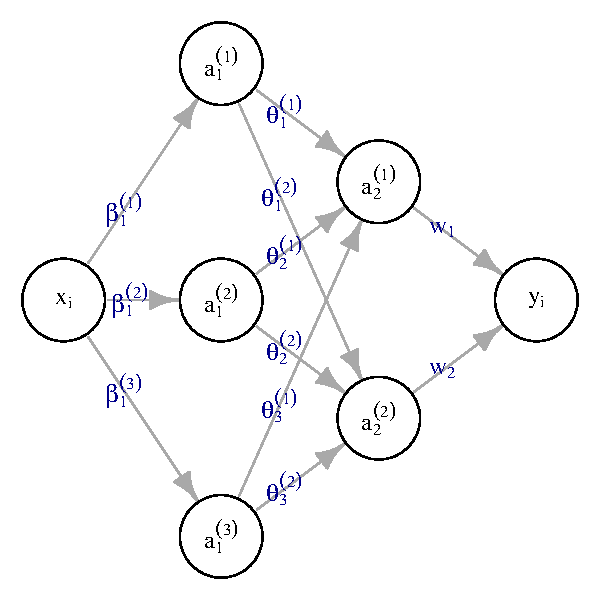
\includegraphics[width=0.6\textwidth]{plot_ANN_02.pdf}
    \caption{Diagram of a multilayer perceptron with two hidden layers, $m = 3$ and $r = 2$.}
    \label{fig:theory_ANN_diagram_02}
\end{figure}

Now that we have a grasp of how the MLP works, we can define it more generally. The notation used will be $y$ for the response variable $n$-dimensional vector, $y_i$ for the $i$-th element of $y$ and $X$ for the data matrix, such that $X \in \mathbb{R}^{n \times p}$, $x_i \in \mathbb{R}^p$ denotes the $i$-th row in $X$ and it represents the values of the covariates for the $i$-th element in the data and $x^{(k)} \in \mathbb{R}^n$ denotes the $k$-th column in $X$. Since a multilayer perceptron can have any integer number of hidden layers, we will denote the number of layers by $L$, the number of nodes of each layer $l$ by $n^{[l]}$ and the activation function for each layer $l$ by $\sigma^{[l]}(\cdot)$, for $l \in \left\{ 1, \ldots, L \right\}$. The activation function for the last layer will be denoted by $\phi(\cdot)$, as in the binary classification example.
The parameter, or weight, for the $k$-th node in the $l$-th layer that connects the $j$-th node from the $(l-1)$-th layer is denoted by $\theta_{j,k}^{[l]}$ and, as before, $a_k^{[l]}$ denotes the result of the activation function corresponding to the $l$-th layer for $k \in \left\{ 1, \ldots, n^{[l]} \right\}$; where $\theta_0^{[l]}$ is the bias term of the $l$-th layer. That is,
$$
  a_k^{[l]} = \sigma^{[l]} \left( \theta_0^{[l]} + \sum_{j = 1}^{n^{[l-1]}} \theta_{j,k}^{[l]} a_j^{(l-1)} \right)
$$

for $k \in \left\{ 1, \ldots, n^{[l]} \right\}$, $j \in \left\{ 1, \ldots, n^{[l-1]} \right\}$ and $l \in \left\{ 1, \ldots, L \right\}$. The value of $a_k^{[0]}$ is the value of the covariate $x^{[k]}$, $a_0^{[0]}$ is a vector of ones of dimension $n$ and $n^{[0]}$ is the number of covariates plus 1, i.e., $n^{[0]} = p + 1$.

\section{Convolutional Neural Networks}

\section{Variational Inference}

\section{Active Learning}
